\subsubsection{AlexNet}\label{alexnet}
When the AlexNet architecture was published in 2012 \citep{AlexNetoriginal}, it (re-)~ignited the field of Deep Learning. An illustration of the network's architecture as presented by Krizhevsky et al\@. in the original paper introducing AlexNet to the world is given in Figure~\ref{fig:alexnet}. At the time, AlexNet was unusually deep, with eight layers in total, consisting of five convolutional layers and three fully connected layers. Back then, a network with this many layers represented a big computational challenge. The authors describe how the training using 90 cycles with a training set of 1.2 million images and using two NVIDIA GTX 580 3GB GPUs took five to six days. Part of the new look consisted of the use of the Rectified Linear Unit (ReLU) function as the activation function and using dropout. The Rectified Linear Unit superseded the previously used tanh activation function. Using ReLU as opposed to tanh enabled the network to be trained several times faster. For the dropout method, the output of each hidden neuron is set to zero according to a probability~-~in the case of the original AlexNet paper 0.5 was chosen \citep{AlexNetoriginal}. The neurons which are subject to having their weight set to zero subsequently neither participate in the forward pass nor in the backward pass. Generally, the authors describe that dropout is intended to yield a model which learns more robust features, albeit at a cost of leading the iterations needed to converge to almost double. However, Krizhevsky et al\@. state that without dropout their network would exhibit substantial overfitting.
\begin{figure}[h]
	\centering
	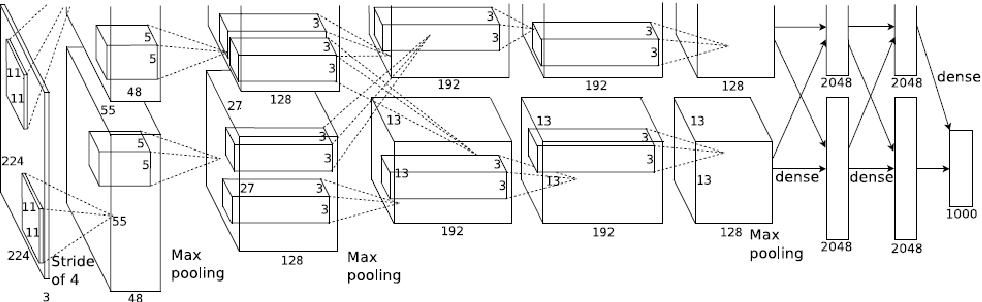
\includegraphics[scale=0.4]{./figures/AlexNet-architecture.png}
	\caption{Original AlexNet architecture}~\label{fig:alexnet}
\end{figure}

